\section{Root-finding decomposition}\label{sec:rootfinding}

\subsection{Origin: a suggestion in an audited manuscript}

The textbook decomposition oracle builds Semaev's polynomial system and
solves it with a Gr\"obner-basis engine. On 12 October a 13-page manuscript,
\emph{Point Decomposition by Root Finding}, was supplied for assessment. We
froze it (\art{research/ecbench_rootfinding_assessment_20261012/source-paper.pdf},
SHA-256 \texttt{743d3d3e\ldots7c01}) and audited it against its source
branch before measuring anything. Its central suggestion is simple: for two
summands, fixing one factor-base point turns $\Sem3$ into a quadratic in the
remaining variable whose roots are already known.

\begin{proposition}[roots of $\Sem3$]\label{prop:s3}
Let $E: y^2=x^3+ax+b$ over a field $K$ of characteristic $\ne2,3$, and let
$R,F\in E(K)$ be affine with $x_R\ne x_F$. Then
\[
  \Sem3(x_R,x_F,X)=(x_R-x_F)^2\,(X-x_+)(X-x_-),\qquad
  x_\pm=x(R\pm F),
\]
so $\Sem3(x_R,x_F,X)=0$ iff $X\in\{x(R+F),x(R-F)\}$.
\end{proposition}
\begin{proof}[Proof sketch]
With $\lambda_\pm=(\pm y_F-y_R)/(x_F-x_R)$ the chord slopes,
$x_\pm=\lambda_\pm^2-x_R-x_F$. Expanding $(X-x_+)(X-x_-)$ and eliminating
$y_R^2,y_F^2$ with the curve equation gives exactly Semaev's
$\Sem3/(x_R-x_F)^2$. The identity is machine-checked over an arbitrary
field in Lean 4 with Mathlib (\art{papers/rootfinding-decomposition/lean/S3Roots.lean},
theorems \texttt{SemaevS3.S3\_factor} and \texttt{SemaevS3.S3\_root\_iff};
no \texttt{sorry}; axioms \texttt{propext}, \texttt{Classical.choice},
\texttt{Quot.sound}).
\end{proof}

Hence the two-summand system has a parametrised variety: $R=\pm F_i\pm F_j$
iff $x(R\mp F_i)\in x(\Fb)$. No polynomial system is solved; the oracle is
one subtraction and one table probe per base point.

\paragraph{What the audit kept and corrected.} The identity is exact under
the stated generic affine condition, and a returned witness can be re-added
in the group for soundness. Completeness of the exhaustive enumeration
holds only with an explicit sign and factor-base convention (the binary
table stores full point keys over a base containing both signs; the
manuscript's schematic $x$-only table needed that convention stated). The
manuscript's NIST baseline was Buchberger, not F4
(\S\ref{sec:corrections}), and its statement that no implementation can
use fewer than linear field operations per ideal fails for repeated
queries against a reusable pair table. Larger-summand enumeration has a
growing exponent in $\abs\Fb$, and the manuscript did not benchmark it end
to end. All of this is recorded in
\art{research/ecbench_rootfinding_assessment_20261012/REPORT.md}.

\subsection{The algorithms}

\begin{algorithm}[t]
\caption[]{Prime two-summand oracle by direct subtraction}\label{alg:prime}
\begin{algorithmic}[1]
\Require target $R$, base $\Fb=\{F_1,\ldots,F_N\}$, hash set $H$ of
abscissae (or full points) of $\Fb$
\State $d_i\gets x_R-x_{F_i}$ for all $i$; invert all $d_i$ with one
  field inversion and $3(N-1)$ multiplications (Montgomery's trick)
\For{$i=1..N$}
  \For{$\varepsilon\in\{+1,-1\}$}
    \State $\lambda\gets(y_R+\varepsilon y_{F_i})\,d_i^{-1}$;\quad
           $x_3\gets\lambda^2-x_R-x_{F_i}$ \Comment{$x(R-\varepsilon F_i)$}
    \If{$x_3\in H$} recover the sign of $F_j$ from $y_3$; emit
      $R=\varepsilon F_i+\tau F_j$ \EndIf
  \EndFor
\EndFor
\end{algorithmic}
\end{algorithm}

\emph{Prime fields} (Algorithm~\ref{alg:prime},
\art{src/cryptanalysis/prime_fast.rs}): $\Theta(N)$ field operations and
$2N$ lookups per target. \emph{Binary fields}
(\art{src/cryptanalysis/koblitz_index_calculus.rs},
\texttt{DecompositionStrategy::PairTable}, made the default): a precomputed
table of pair sums $F_i+F_j$ turns an $m$-decomposition into $1$, $N$ or
$N^2$ lookups for $m=2,3,4$---the meet-in-the-middle half of a birthday
search, exact and complete like exhaustive search, at the price of
$\Theta(N^2)$ set-up and memory. Both are verified fail closed: every
decomposition is re-added in the group, $\Sem3$ is checked to vanish,
Gr\"obner-variety membership and agreement on refutation are checked
against F4, and planted positive controls must be found.

\subsection{Generalising the observation}

Over three days the identity was carried through every layer of the
pipeline. Table~\ref{tab:rf-steps} lists the steps; each is its own study
with a protocol registered before it ran.

\begin{table}[t]
\centering\small
\caption[]{Root-finding generalisations, 12--14 October. Every row is
\cls{engineering}: no slope fell below its generic floor.}
\label{tab:rf-steps}
\begin{tabularx}{\linewidth}{@{}>{\raggedright}p{3.1cm}X@{}}
\toprule
Step & What it adds; artefact \\
\midrule
Prime subtraction, binary pair table &
  Prop.~\ref{prop:s3}; batched inversion; $m\le4$ tables.
  \art{research/semaev_root_vs_groebner_20261012/} \\
NIST P-192\ldots P-521 &
  standard parameters, 6- and 64-point bases; dedicated P-256 field
  $11$--$12\times$ over generic big integers.
  \art{research/semaev_rootfind_nist_20261012/} \\
End to end vs msolve &
  complete DLPs with only the oracle swapped.
  \art{research/semaev_rootfind_e2e_20261012/} \\
PDP oracle family &
  \texttt{rf-mitm}, \texttt{mitm3}, \texttt{mitm4} (2-sum table);
  \texttt{rf-pairs}, \texttt{pairs3} (pairs then solve by the group law);
  \texttt{subtract2}; binary rungs $\ell=8..14$, prime Kummer towers
  $m=2,3,4$. \art{research/pdp_root_finder_20261012/} \\
CUDA kernel &
  one thread per (target, slice); per-thread Montgomery inversion; SoA
  base; shared-memory hash for $\abs\Fb\le2048$; 64-bit and P-256 fields.
  Validated in host emulation only (no GPU available).
  \art{RESEARCH_GPU_ROOTFIND_DECOMPOSITION.md} \\
ecbench engines &
  \texttt{pdp3-koblitz:m=2|3,engine=rootfind}, \texttt{rootfind-subtract},
  later \texttt{rootfind-window} and \texttt{rootfind-negfold}.
  \art{research/ecbench_rootfind_engine_20261012/} and successors \\
Kummer-tower base &
  PKM's $\mu_{2^t}$ base with the root-finding oracles, 20--28-bit primes.
  \art{research/pkm_tower_ecbench_20261013/} \\
Dense root index, $n=83$ &
  packed five-byte $\Sem3$ root table, prefix widths K1271--K1798,
  8\,GiB of slots. \art{research/n83_dense_root_20261013/} \\
Prime tuning &
  pair-table size, arity, batched table inversions, synchronised lanes.
  \art{research/ecbench_rootfinding_\{tuning,arity,batchtable,lanes\}_2026101*/} \\
\bottomrule
\end{tabularx}
\end{table}

\subsection{Results}

\begin{figure}[t]
\centering
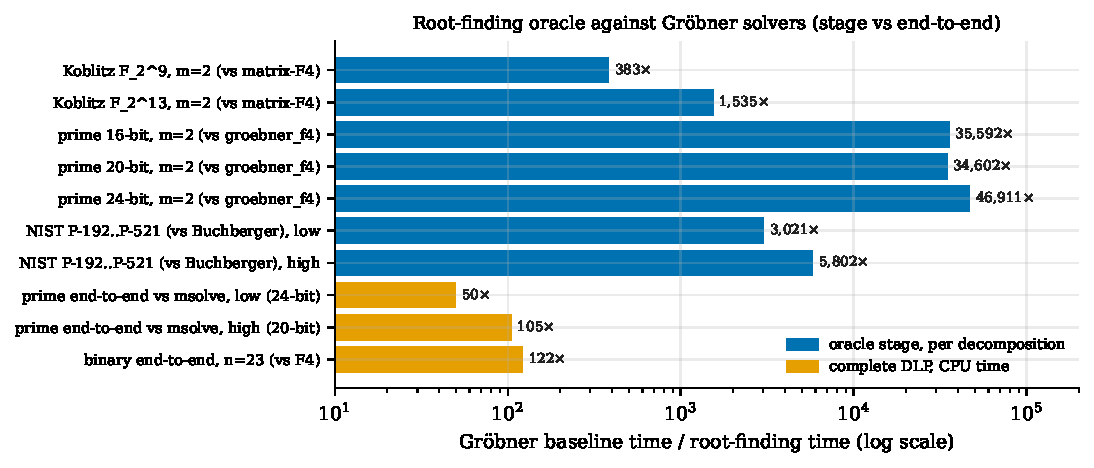
\includegraphics[width=\linewidth]{figures/fig-rootfind-oracle.pdf}
\caption[]{Root finding against Gr\"obner solvers on identical targets. Blue:
one decomposition (oracle stage only). Orange: complete discrete-log
computations with the oracle swapped and everything else fixed (prime: CPU
time against msolve, 20/24-bit totals composed from sampled per-query cost;
binary: one cold solve including table build). Sources:
\art{RESEARCH_SEMAEV_ROOTFIND_VS_GROEBNER.md},
\art{papers/rootfinding-decomposition/README.md}.}
\label{fig:rf-oracle}
\end{figure}

\paragraph{Oracle stage.} Per decomposition, root finding is
$383\times$ ($\FF_{2^9}$, $\abs\Fb=55$, 254 targets) and $1{,}535\times$
($\FF_{2^{13}}$, $\abs\Fb=4{,}005$, 256 targets) faster than matrix F4;
$3.5$--$4.7\cdot10^4\times$ faster than \texttt{groebner\_f4} on 16--24-bit
prime curves ($\abs\Fb=6$, 40 targets each); and $3{,}021$--$5{,}802\times$
faster than Buchberger on the decomposition ideal of the five NIST curves
(Figure~\ref{fig:rf-oracle}). Every binary verdict agreed with F4; every
prime solution was in F4's variety and every prime refutation was F4's unit
ideal. In the PDP study, \texttt{rf-mitm} refutes a binary target in
$3.1\,\mu$s at $\ell=8$ and $482\,\mu$s at $\ell=14$, against the PS-0
baseline's $9.3$\,ms and $55.5$\,s ($3{,}007$--$115{,}160\times$), costs
$5\abs\Fb-3$ multiplications and $2\abs\Fb$ lookups a target, and sits on
the pair-table floor at $1.000\pm0.027$ bits per rung; at prime $m=3$,
$N=18$ it uses 197 multiplications where F4 uses $8.99\cdot10^{13}$
multiply-adds; 707/707 brute-force agreements
(\art{research/pdp_root_finder_20261012/}).

\paragraph{Complete solves.} End to end, the gain is two orders of
magnitude smaller and not one-sided: $50$--$105\times$ against msolve on
16--24-bit prime curves; $122\times$ on the one binary instance ($n=23$)
large enough to amortise the pair table; and F4 \emph{faster} at
$n=5,9,13$, where a solve needs too few decompositions to pay for the
table. Inside ecbench, with every group operation charged, the
root-finding IC beats inherited F4 in solve wall by about $350\times$ at
$n=13$ (admitted) and about $10^4\times$ at $n=23$ (descriptive), yet stays
$2.9$--$25{,}116\times$ the strong rho in $S$ on binary curves and
$29$--$141\times$ rho on prime curves, with the gap widening
(\art{research/pdp_root_finder_ecbench_20261013/}).

\paragraph{The Koblitz loops.} Figure~\ref{fig:k13} follows the best
complete-count root-finding arm at Koblitz $E_0$, $n=13$ through four
registered improvement loops (8 public targets $\times$ 3 rounds each, L0
operation counts). The first engine had $S=38.82$ ($m=3$) and $28.38$
($m=2$). A windowed third-summand scan cut $m=3$ by a paired $0.828$
$[0.783,0.863]$; a fold over negation (\texttt{rootfind-negfold}) took
$m=2$ to $23.22$ and then $22.97$. Two further cycles of denser and
sparser bases, windowed negfold and plain root finding were dead ends
(\art{research/ecbench_rootfind_vs_rho_20261014/}). With F4's word XORs
priced, the paired ratio negfold/F4 is $0.0545$ $[0.047,0.064]$, a
complete-against-complete comparison; against strong signed-Frobenius rho
($S=14.82$) the best complete arm is still $1.55\times$. A compact-orbit
base with a counted Frobenius pair table reaches $S=15.55$, below the
then-unpriced F4 ($16.75$), but it is itself a lower bound
(factor-base construction natives unpriced), and it is $1.08\times$ rho.
Amortised over 64 targets that arm reaches $S\approx11.2$, below rho; by
the ledger's rules that is a secondary, multi-target result, not a cold
claim.

\begin{figure}[t]
\centering
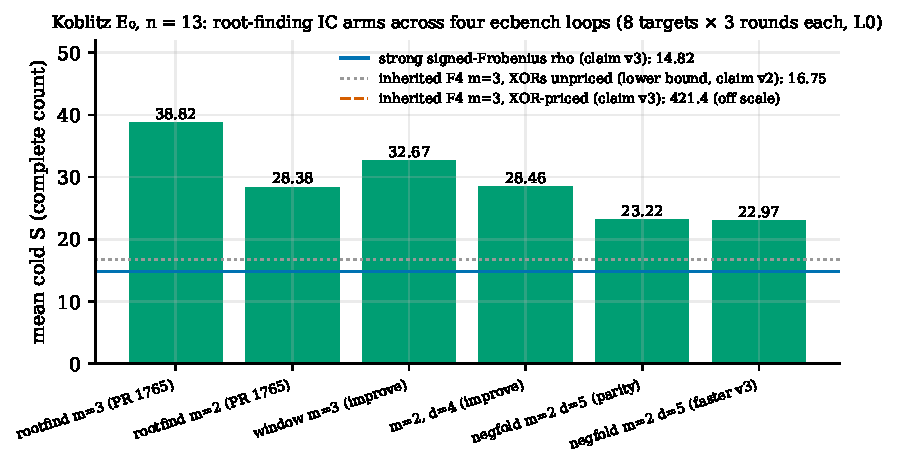
\includegraphics[width=\linewidth]{figures/fig-k13-progression.pdf}
\caption[]{Mean cold $S$ of root-finding IC arms at Koblitz $E_0$, $n=13$,
$d=5$ unless stated, across the engine, improve, parity and faster loops.
All bars are complete counts. Sources:
\art{research/ecbench_rootfind_engine_20261012/},
\art{research/ecbench_rootfind_improve_20261013/},
\art{research/ecbench_rootfind_parity_20261013/},
\art{research/ecbench_rootfind_faster_20261014/}. Each loop had its own
seeds and rho arm (rho $14.12$--$14.82$).}
\label{fig:k13}
\end{figure}

\paragraph{Prime tuning in ecbench.} On a 20-bit prime curve, the pair
table's counted $S$ is $0.018861$ $[0.018547,0.019242]$ of direct
subtraction (24 pairs; prime native work unpriced, so a bounded ratio), and
$0.057047$ $[0.041159,0.092069]$ on a 17-bit Koblitz curve, fully priced,
where the table set-up is about 68\% of the arm's cold cost. Doubling the
table from 32 to 64 abscissae gives $0.830$ $[0.697,0.962]$; three
summands instead of two costs $1.431\times$ $[1.225,1.716]$; batching the
table inversions leaves counted GAE unchanged ($1.000$; $4{,}096$ versus
$64$ inversions, set-up wall $243$ versus $128\,\mu$s, descriptive); and a
train-set lane selection did not resolve a hold-out winner ($0.979$
$[0.919,1.038]$; 1{,}088/1{,}088 verified executions)
(\art{benchmarks/README.md}, rows of 12--14 Oct).

\paragraph{Dense root index at $n=83$.} Widening the prefix base from
K1500 to K1798 cut mean probes per relation from $300{,}021.9$ to
$169{,}069.8$ (paired difference $130{,}952$, 95\% $[52{,}058,209{,}991]$)
and gave a one-point online ratio of $18.528$ over same-point rho (IC
$63.3$\,ms, rho $1{,}173.3$\,ms), with $339.0$\,s of reusable preparation
and an 8\,GiB table outside the window. The host was shared, so the result
is exploratory; two K1500 runs hit the 900\,s timeout and are retained.

\paragraph{Reading.} Root finding is the largest constant-factor change
of the programme at the oracle stage, and the one with a proof behind it.
It does not change the asymptotic count of index calculus: its cost is
$\Theta(\abs\Fb^{m-1})$, every measurement is at $m\le4$, and it leaves
relation yield, factor-base size and linear algebra untouched. Its effect
on the cold frontier is to move the decomposition stage from dominant to
minor, which exposes the stages that now are.
